\section{Recurrent Neural Networks}\label{sec:rnn}

So far we encountered two types of data: generic vectors and images. For the latter we designed specialized layers to take advantage of the regularity properties in them. Besides, we tacitly assumed that our data is generated i.i.d., i.e. independently and identically distributed, all drawn from some distribution. Unfortunately, this is not true for many types of data. For instance, the words in this paragraph are written in sequence, and it would be quite difficult to decipher its meaning if they were permuted randomly. Likewise, image frames in a video, the audio signal in a conversation, or the browsing behavior on a website, all follow sequential order. It is thus only reasonable to assume that specialized models for such data will do better at describing it and at solving estimation problems.

Another issue arises from the fact that we might not only receive a sequence as an input but rather might be expected to continue the sequence. For instance, the task could be to continue the series 2, 4, 6, 8, 10, … This is quite common in time series analysis, to predict the stock market, the fever curve of a patient or the acceleration needed for a race car. Again we want to have models that can handle such data.

In short, while convolutional neural networks can efficiently process spatial information, recurrent neural networks are designed to better handle sequential information. These networks introduces state variables to store past information and, together with the current input, determine the current output.

Many of the examples for using recurrent networks are based on text data. Hence, we will emphasize language models in this chapter. After a more formal review of sequence data we discuss basic concepts of a language model and use this discussion as the inspiration for the design of recurrent neural networks. Next, we describe the gradient calculation method in recurrent neural networks to explore problems that may be encountered in recurrent neural network training. For some of these problems, we can use gated recurrent neural networks, such as LSTMs and GRUs, described later in this section.

\subsection{Sequence models}\label{subsec:sequence_models}

There many examples of observable behaviour and phenomena that are sequential in nature, that is, that change over time. In mathematics, a sequence is a list of objects (or events) which have been fully ordered, such that each member either comes before, or after, every other member. More formally, a sequence is a function with a domain equal to the set of positive integers.

In short, we need statistical tools and new deep networks architectures to deal with sequence data. To keep things simple, we use stock prices as an example (see \cref{fig:ftse100}).

\begin{figure}[hpt]
	\centering
	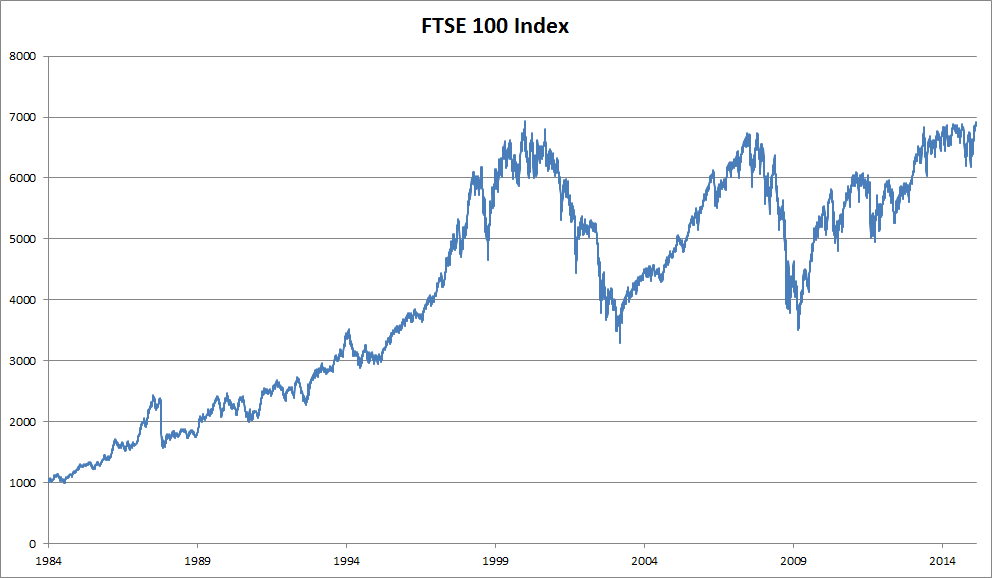
\includegraphics[scale=0.5]{images/ch3/ftse100.png}
	\caption{FTSE 100 index over 30 years.}
	\label{fig:ftse100}
\end{figure}

Let’s denote the prices by $x_t \geq 0$, i.e. at time $t \in \mathbb{N}$ we observe some price $x_t$. For a trader to do well in the stock market on day $t$ he should want to predict $x_t$ via

$$x_t \sim p(x_t|x_{t-1}, \ldots x_1)$$

\subsubsection{Autoregressive Models}

In order to achieve this, our trader could use a regressor, but there’s just a major problem - the number of inputs, $x_{t-1}, \ldots x_1$ varies, depending on $t$. That is, the number increases with the amount of data that we encounter, and we will need an approximation to make this computationally tractable. Much of what follows in this section will revolve around how to estimate $p(x_t|x_{t-1}, \ldots x_1)$ efficiently. In a nutshell it boils down to two strategies:

\begin{enumerate}
    \item Assume that the potentially rather long sequence $x_{t-1}, \ldots x_1$ is not really necessary. In this case we might content ourselves with some timespan $\tau$ and only use $x_{t-1}, \ldots x_{t-\tau}$ observations. The immediate benefit is that now the number of arguments is always the same, at least for $t > \tau$. This allows us to train a deep network as indicated above. Such models will be called \textit{autoregressive models}, as they quite literally perform regression on themselves.
    \item Another strategy is to try and keep some summary $h_t$ of the past observations around and update that in addition to the actual prediction. This leads to models that estimate $x_t|x_{t-1}, h_{t-1}$ and moreover updates of the form $h_t = g(h_t, x_t)$. Since $h_t$ is never observed, these models are also called \textit{latent autoregressive models}. LSTMs and GRUs are examples of this.
\end{enumerate}

Both cases raise the obvious question of how to generate training data. One typically uses historical observations to predict the next observation given the ones up to right now. Obviously we do not expect time to stand still. However, a common assumption is that while the specific values of $x_t$ might change, at least the dynamics of the time series itself won’t. This is reasonable, since novel dynamics are just that, novel and thus not predictable using data we have so far. Statisticians call dynamics that do not change stationary. Regardless of what we do, we will thus get an estimate of the entire time series via

$$p(x_1, \ldots x_T) = \prod_{t=1}^T p(x_t|x_{t-1}, \ldots x_1)$$

Note that the above considerations still hold if we deal with discrete objects, such as words, rather than numbers. The only difference is that in such a situation we need to use a classifier rather than a regressor to estimate $p(x_t| x_{t-1}, \ldots x_1)$.

\subsubsection{Markov Model}

Recall the approximation that in an autoregressive model we use only $(x_{t-1}, \ldots x_{t-\tau})$ instead of $(x_{t-1}, \ldots x_1)$ to estimate $x_t$. Whenever this approximation is accurate we say that the sequence satisfies a Markov condition. In particular, if $\tau = 1$, we have a first order Markov model and $p(x)$ is given by

$$p(x_1, \ldots x_T) = \prod_{t=1}^T p(x_t|x_{t-1})$$

Such models are particularly nice whenever $x_t$ assumes only discrete values, since in this case dynamic programming can be used to compute values along the chain exactly. For instance, we can compute $x_{t+1}|x_{t-1}$ efficiently using the fact that we only need to take into account a very short history of past observations.

$$p(x_{t+1}|x_{t-1}) = \sum_{x_t} p(x_{t+1}|x_t) p(x_t|x_{t-1})$$

Going into details of dynamic programming is beyond the scope of this section. Control and reinforcement learning algorithms use such tools extensively.

\subsubsection{Causality}

In principle, there’s nothing wrong with unfolding $p(x_1, \ldots x_T)$ in reverse order. After all, by conditioning we can always write it via

$$p(x_1, \ldots x_T) = \prod_{t=T}^1 p(x_t|x_{t+1}, \ldots x_T)$$

In fact, if we have a Markov model we can obtain a reverse conditional probability distribution, too. In many cases, however, there exists a natural direction for the data, namely going forward in time. It is clear that future events cannot influence the past. Hence, if we change $x_t$, we may be able to influence what happens for $x_{t+1}$ going forward but not the converse. That is, if we change $x_t$, the distribution over past events will not change. Consequently, it ought to be easier to explain $x_{t+1}|x_t$ rather than $x_t|x_{t+1}$. For instance, \citet{Hoyer2008} show that in some cases we can find $x_{t+1} = f(x_t) + \epsilon$ for some additive noise, whereas the converse is not true. This is great news, since it is typically the forward direction that we’re interested in estimating. For more on this topic see for example the book \textit{Elements of Causal Inference}, by \citet{Peters2015}; we are barely scratching the surface of it.

\subsection{Language models}\label{subsec:lang_models}

Text is an important example of sequence data. In fact, we will use natural language models as the basis for many of the examples in this chapter. Given that, it’s worth while discussing some things in a bit more detail. In the following we will view words (or sequences of characters) as a time series of discrete observations. Assuming the words in a text of length $T$ are in turn $w_1, w_2, \ldots, w_T$, then, in the discrete time series, $w_t(1 \leq t \leq T)$ can be considered as the output or label of time step $t$. Given such a sequence, the goal of a language model is to estimate the probability

$$p(w_1, w_2, \ldots, w_T)$$

Language models are incredibly useful. For instance, an ideal language model would be able to generate natural text just on its own, simply by drawing one word at a time $w_t \sim p(w_t|w_{t-1}, \ldots w_1)$. Quite unlike the monkey using a typewriter, all text emerging from such a model would pass as natural language, e.g. English text. Furthermore, it would be sufficient for generating a meaningful dialog, simply by conditioning the text on previous dialog fragments. Clearly we are still very far from designing such a system, since it would need to understand the text rather than just generate grammatically sensible content.

Nonetheless language models are of great service even in their limited form. For instance, the phrases ‘to recognize speech’ and ‘to wreck a nice beach’ sound very similar. This can cause ambiguity in speech recognition, ambiguity that is easily resolved through a language model which rejects the second translation as outlandish. Likewise, in a document summarization algorithm it’s worth while knowing that ‘dog bites man’ is much more frequent than ‘man bites dog’, or that ‘let’s eat grandma’ is a rather disturbing statement, whereas ‘let’s eat, grandma’ is much more benign.

\subsubsection{Estimating a language model}

The obvious question is how we should model a document, or even a sequence of words. We can start by applying basic probability rules:

$$p(w_1, w_2, \ldots, w_T) = \prod_{t=1}^T p(w_t | w_1, \ldots, w_{t-1})$$

For example, the probability of a text sequence containing four tokens consisting of words and punctuation would be given as:

$$p(\mathrm{Statistics}, \mathrm{is},  \mathrm{fun}, \mathrm{.}) =  p(\mathrm{Statistics}) p(\mathrm{is} | \mathrm{Statistics}) p(\mathrm{fun} | \mathrm{Statistics}, \mathrm{is}) p(\mathrm{.} | \mathrm{Statistics}, \mathrm{is}, \mathrm{fun})$$

In order to compute the language model, we need to calculate the probability of words and the conditional probability of a word given the previous few words, i.e. language model parameters. Here, we assume that the training data set is a large text corpus, such as all Wikipedia entries, Project Gutenberg, or all text posted online on the web. The probability of words can be calculated from the relative word frequency of a given word in the training data set.

For example, $p(\mathrm{Statistics})$ can be calculated as the probability of any sentence starting with the word ‘statistics’. A slightly less accurate approach would be to count all occurrences of the word ‘statistics’ and divide it by the total number of words in the corpus. This works fairly well, particularly for frequent words. Moving on, we could attempt to estimate

$$\hat{p}(\mathrm{is}|\mathrm{Statistics}) = \frac{n(\mathrm{Statistics~is})}{n(\mathrm{Statistics})}$$

Here $n(w)$ and $n(w, w')$ are the number of occurrences of singletons and pairs of words respectively. Unfortunately, estimating the probability of a word pair is somewhat more difficult, since the occurrences of ‘Statistics is’ are a lot less frequent. In particular, for some unusual word combinations it may be tricky to find enough occurrences to get accurate estimates. Things take a turn for the worse for 3 word combinations and beyond. There will be many plausible 3-word combinations that we likely will not see in our dataset. Unless we provide some solution to give such word combinations nonzero weight we will not be able to use these as a language model. If the dataset is small or if the words are very rare, we might not find even a single one of them.

A common strategy is to perform some form of Laplace smoothing, that is, adding a small constant to all counts. 
%This helps with singletons, e.g. via

% $$
% \begin{aligned}
%     \hat{p}(w) & = \frac{n(w) + \epsilon_1/m}{n + \epsilon_1} \\
%     \hat{p}(w'|w) & = \frac{n(w,w') + \epsilon_2 \hat{p}(w')}{n(w) + \epsilon_2} \\
%     \hat{p}(w''|w',w) & = \frac{n(w,w',w'') + \epsilon_3 \hat{p}(w',w'')}{n(w,w') + \epsilon_3}
% \end{aligned}
% $$

% Here the coefficients $\epsilon_i > 0$ determine how much we use the estimate for a shorter sequence as a fill-in for longer ones. Moreover, $m$ is the total number of words we encounter. The above is a rather primitive variant of what Kneser-Ney smoothing and Bayesian Non-parametrics can accomplish. 

See e.g. \textit{The Sequence Memoizer} by \citep{Wood2011} for more details of how to accomplish this. Unfortunately models like this get unwieldy rather quickly. First off, we need to store all counts and secondly, this entirely ignores the meaning of the words; for instance, ‘cat’ and ‘feline’ should occur in related contexts. Besides, it is quite difficult to adjust such models to additional context. Lastly, long word sequences are almost certain to be novel, hence a model that simply counts the frequency of previously seen word sequences is bound to perform poorly there.

\subsubsection{Markov Models and n-grams}

Before we discuss solutions involving deep learning we need some more terminology and concepts. Recall our discussion of Markov Models in the previous section. Let’s apply this to language modeling. A distribution over sequences satisfies the Markov property of first order if $p(w_{t+1}|w_t, \ldots w_1) = p(w_{t+1}|w_t)$. Higher orders correspond to longer dependencies. This leads to a number of approximations that we could apply to model a sequence:

$$
\begin{aligned}
p(w_1, w_2, w_3, w_4) &=  p(w_1) p(w_2) p(w_3) p(w_4)\\
p(w_1, w_2, w_3, w_4) &=  p(w_1) p(w_2 | w_1) p(w_3 | w_2) p(w_4 | w_3)\\
p(w_1, w_2, w_3, w_4) &=  p(w_1) p(w_2 | w_1) p(w_3 | w_1, w_2) p(w_4 | w_2, w_3)\\
\end{aligned}
$$

Since they involve one, two or three terms, these are typically referred to as \textit{unigram}, \textit{bigram} and \textit{trigram} models. 
% In the following we will learn how to design better models.

\subsection{Recurrent Neural Networks}\label{subsec:rnn}

In the previous section we introduced $n$-gram models, where the conditional probability of word $w_t$ at position $t$ only depends on the $n-1$ previous words. If we want to check the possible effect of words earlier than $t-(n-1)$ on $w_t$, we need to increase $n$. However, the number of model parameters would also increase exponentially with it, as we need to store $|V|^n$ numbers for a vocabulary $V$. Hence, rather than modeling $p(w_t|w_{t-1}, \ldots w_{t-n+1})$ it is preferable to use a latent variable model in which we have

$$p(w_t|w_{t-1}, \ldots w_1) \approx p(w_t|h_t(w_{t-1}, h_{t-1})).$$

For a sufficiently powerful function $h_t$ this is not an approximation. After
all, $h_t$ could simply store all the data it observed so far. We discussed this
in \cref{subsec:sequence_models}. Let's see why building such models is a bit more tricky than simple autoregressive models where

$$p(w_t|w_{t-1}, \ldots w_1) \approx p(w_t|f(w_{t-1}, \ldots w_{t-n+1}))$$

As a warmup we will review the latter for discrete outputs and $n=2$, i.e. for Markov model of first order. To simplify things further we use a single layer in the design of the RNN. Later on we will see how to add more expressivity efficiently across items.

\subsubsection{Recurrent Networks Without Hidden States}

Let us take a look at a multilayer perceptron with a single hidden layer. Given a mini-batch of instances $\mathbf{X} \in \mathbb{R}^{n \times d}$ with sample size $n$ and $d$ inputs (features or feature vector dimensions). Let the hidden layer's activation function be $\phi$. Hence the hidden layer's output $\mathbf{H} \in \mathbb{R}^{n \times h}$ is calculated as

$$\mathbf{H} = \phi(\mathbf{X} \mathbf{W}_{xh} + \mathbf{b}_h).$$

Here, we have the weight parameter $\mathbf{W}_{xh} \in \mathbb{R}^{d \times h}$, bias parameter $\mathbf{b}_h \in \mathbb{R}^{1 \times h}$, and the number of hidden units $h$, for the hidden layer. 
% Recall that $\mathbf{b}_h$ is just a vector - its values are replicated using the broadcasting mechanism to match those of the matrix-matrix product.

Also note that hidden \textbf{state} and hidden \textbf{layer} refer to two very different concepts. Hidden layers are layers that are hidden from view on the path from input to output. Hidden states are technically speaking inputs to whatever we do at a given step. Instead, they can only be computed by looking at data at previous iterations. In this sense they have much in common with latent variable models in statistics, such as clustering or topic models where e.g. the cluster ID affects the output but cannot be directly observed.

The hidden variable $\mathbf{H}$ is used as the input of the output layer. For classification purposes, such as predicting the next character, the output dimensionality $q$ might e.g. match the number of categories in the classification problem. Lastly the output layer is given by

$$\mathbf{O} = \mathbf{H} \mathbf{W}_{hq} + \mathbf{b}_q.$$

Here, $\mathbf{O} \in \mathbb{R}^{n \times q}$ is the output variable, $\mathbf{W}_{hq} \in \mathbb{R}^{h \times q}$ is the weight parameter, and $\mathbf{b}_q \in \mathbb{R}^{1 \times q}$ is the bias parameter of the output layer.  If it is a classification problem, we can use $\text{softmax}(\mathbf{O})$ to compute the probability distribution of the output category. This is entirely analogous to the regression problem we solved previously in \cref{subsec:sequence_models}, hence we omit details. Suffice it to say that we can pick $(w_t, w_{t-1})$ pairs at random and estimate the parameters $\mathbf{W}$ and $\mathbf{b}$ of our network via autograd and stochastic gradient descent.

\subsubsection{Recurrent Networks with Hidden States}\label{subsubsec:rnn_with_hidden_state}

Matters are entirely different when we have hidden states. Let's look at the structure in some more detail. Assume that $\mathbf{X}_t \in \mathbb{R}^{n \times d}$ is the mini-batch input and $\mathbf{H}_t  \in \mathbb{R}^{n \times h}$ is the hidden variable of time step $t$ from the sequence.  Unlike the multilayer perceptron, here we save the hidden variable $\mathbf{H}_{t-1}$ from the previous time step and introduce a new weight parameter $\mathbf{W}_{hh} \in \mathbb{R}^{h \times h}$, to describe how to use the hidden variable of the previous time step in the current time step. Specifically, the calculation of the hidden variable of the current time step is determined by the input of the current time step together with the hidden variable of the previous time step:

$$\mathbf{H}_t = \phi(\mathbf{X}_t \mathbf{W}_{xh} + \mathbf{H}_{t-1} \mathbf{W}_{hh}  + \mathbf{b}_h)$$

Compared with the multilayer perceptron, we added one more $\mathbf{H}_{t-1} \mathbf{W}_{hh}$ here. From the relationship between hidden variables $\mathbf{H}_t$ and $\mathbf{H}_{t-1}$ of adjacent time steps, we know that those variables captured and retained the sequence's historical information up to the current time step, just like the state or memory of the neural network's current time step. Therefore, such a hidden variable is also called a hidden state. Since the hidden state uses the same definition of the previous time step in the current time step, the computation of the equation above is recurrent, hence the name recurrent neural network (RNN).

There are many different RNN construction methods.  RNNs with a hidden state defined by the equation above are very common. For time step $t$, the output of the output layer is similar to the computation in the multilayer perceptron:

$$\mathbf{O}_t = \mathbf{H}_t \mathbf{W}_{hq} + \mathbf{b}_q$$

RNN parameters include the weight $\mathbf{W}_{xh} \in \mathbb{R}^{d \times h}, \mathbf{W}_{hh} \in \mathbb{R}^{h \times h}$ of the hidden layer with the bias $\mathbf{b}_h \in \mathbb{R}^{1 \times h}$, and the weight $\mathbf{W}_{hq} \in \mathbb{R}^{h \times q}$ of the output layer with the bias $\mathbf{b}_q \in \mathbb{R}^{1 \times q}$. It is worth mentioning that RNNs always use these model parameters, even for different time steps. Therefore, the number of RNN model parameters does not grow as the number of time steps increases.

\cref{fig:rnn} shows the computational logic of an RNN at three adjacent time steps. In time step $t$, the computation of the hidden state can be treated as an entry of a fully connected layer with the activation function $\phi$ after concatenating the input $\mathbf{X}_t$ with the hidden state $\mathbf{H}_{t-1}$ of the previous time step.  The output of the fully connected layer is the hidden state of the current time step $\mathbf{H}_t$. Its model parameter is the concatenation of $\mathbf{W}_{xh}$ and $\mathbf{W}_{hh}$, with a bias of $\mathbf{b}_h$. The hidden state of the current time step $t$ $\mathbf{H}_t$ will participate in computing the hidden state $\mathbf{H}_{t+1}$ of the next time step $t+1$, the result of which will become the input for the fully connected output layer of the current time step.

\begin{figure}[hpt]
	\centering
	\includesvg[scale=0.5]{images/ch3/rnn.svg}
	\caption{An RNN with a hidden state.}
	\label{fig:rnn}
\end{figure}

As discussed, the computation in the hidden state uses $\mathbf{H}_t = \mathbf{X}_t \mathbf{W}_{xh} + \mathbf{H}_{t-1} \mathbf{W}_{hh}$ to generate an object matching $\mathbf{H}_{t-1}$ in dimensionality. Moreover, we use $\mathbf{H}_t$ to generate the output $\mathbf{O}_t = \mathbf{H}_t \mathbf{W}_{hq}$.

The recurrent network defined above takes observations $X$ and a hidden state $H$ as arguments and uses them to update the hidden state and emit an output $O$. Since this chain could go on for a very long time, training the model with backprop is out of the question (at least without some approximation). After all, this leads to a very long chain of dependencies that would be prohibitive to solve exactly: books typically have more than 100,000 characters and it is unreasonable to assume that the later text relies indiscriminately on all occurrences that happened, say, 10,000 characters in the past. Truncation methods such as BPTT and long short term memory, described later, are useful to address this in a more principled manner. 

\subsubsection{Recurrent networks for language modelling}\label{subsubsec:rnn_lang_modelling}

We conclude this section by illustrating how RNNs can be used to build a language model. For simplicity of illustration we use words rather than characters, since the former are easier to comprehend. Let the number of mini-batch examples be 1, and the sequence of the text be the beginning of our dataset, i.e. “The time Machine by H. G. Wells”. \cref{fig:rnn-train} illustrates how to estimate the next character based on the present and previous characters. During the training process, we run a softmax operation on the output from the output layer for each time step, and then use the cross-entropy loss function to compute the error between the result and the label. Due to the recurrent computation of the hidden state in the hidden layer, the output of time step 3, $\mathbf{O}_3$ is determined by the text sequence “the”, “time”, “machine”. Since the next word of the sequence in the training data is “by”, the loss of time step 3 will depend on the probability distribution of the next word generated based on the sequence “the”, “time”, “machine” and the label “by” of this time step.

\begin{figure}[hpt]
	\centering
	\includesvg[scale=0.8]{images/ch3/rnn-train.svg}
	\caption{Word-level RNN language model. The input and label sequences are The Time Machine by H. and Time Machine by H. G. respectively.}
	\label{fig:rnn-train}
\end{figure}


The number of words is huge compared to the number of characters. This is why quite often we will use a character-level RNN instead.

% \subsection{Text Preprocessing}

% \subsubsection{Tokenization and vocabulary building}

% In the previous section we discussed some properties that make language unique. The key is that the number of tokens (aka words) is large and very unevenly distributed. Hence, a naive multiclass classification approach to predict the next symbol doesn’t always work very well. Moreover, we need to turn text into a format that we can optimize over, i.e. we need to map it to vectors. At its extreme we have two alternatives. One is to treat each word as a unique entity, e.g. \citep{Salton1975}. The problem with this strategy is that we might well have to deal with 100,000 to 1,000,000 vectors for very large and diverse corpora.

% At the other extreme lies the strategy to predict one character at a time, as suggested e.g. by \citet{Ling2015}. A good balance in between both strategies is byte-pair encoding, as described by \citet{Sennrich2016} for the purpose of neural machine translation. It decomposes text into syllable-like fragments that occur frequently. This allows for models that are able to generate words like heteroscedastic or pentagram based on previously viewed words, e.g. heterogeneous, homoscedastic, diagram, and pentagon. Going into details of these models is beyond the scope of the current chapter. 

% Next we need to split the dataset, a string, into tokens. A token is a data point the model will train and predict. We commonly use a word or a character as a token.

% Then we need to map tokens into numerical indices. We often call it a vocabulary. Its input is a list of tokens, called a corpus. Then it counts the frequency of each token in this corpus, and then assigns an numerical index to each token according to its frequency. Rarely appeared tokens are often removed to reduce the complexity. A token doesn’t exist in corpus or has been removed is mapped into a special unknown ("<unk>") token. We optionally add another three special tokens: "<pad>" a token for padding, "<bos>" to present the beginning for a sentence, and "<eos>" for the ending of a sentence.

% \subsubsection{Sampling}

% During training, we need to read mini-batches of examples and labels at random. Since sequence data is by its very nature sequential, we need to address the issue of processing it. Consider the beginning of the book we just processed. If we want to split it up into sequences of 5 symbols each, we have quite some freedom since we could pick an arbitrary offset.

% \begin{figure}[hpt]
% 	\centering
% 	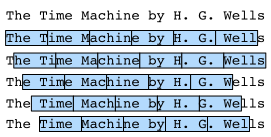
\includegraphics{images/ch3/timemachine-5gram.svg}
% 	\caption{ifferent offsets lead to different subsequences when splitting up text.}
% 	\label{fig:timemachine-5gram}
% \end{figure}

% In fact, any one of these offsets is fine. Hence, which one should we pick? In fact, all of them are equally good. But if we pick all offsets we end up with rather redundant data due to overlap, particularly if the sequences are long. Picking just a random set of initial positions is no good either since it does not guarantee uniform coverage of the array. For instance, if we pick $n$ elements at random out of a set of $n$ with random replacement, the probability for a particular element not being picked is $(1-1/n)^n \to e^{-1}$. This means that we cannot expect uniform coverage this way. Even randomly permuting a set of all offsets does not offer good guarantees. Instead we can use a simple trick to get both coverage and randomness: use a random offset, after which one uses the terms sequentially. This can be done both for random sampling and sequential partitioning.

% \paragraph{Random sampling}

% Randomly generates a minibatch from the data each time. In random sampling, each example is a sequence arbitrarily captured on the original sequence. The positions of two adjacent random mini-batches on the original sequence are not necessarily adjacent. The target is to predict the next character based on what we’ve seen so far, hence the labels are the original sequence, shifted by one character. Note that this is not recommended for latent variable models, since we do not have access to the hidden state prior to seeing the sequence. 

% \paragraph{Sequential partitioning}

% In addition to random sampling of the original sequence, we can also make the positions of two adjacent random mini-batches adjacent in the original sequence. Now, we can use a hidden state of the last time step of a mini-batch to initialize the hidden state of the next mini-batch, so that the output of the next mini-batch is also dependent on the input of the mini-batch, with this pattern continuing in subsequent mini-batches. This has two effects on the implementation of a recurrent neural network. On the one hand, when training the model, we only need to initialize the hidden state at the beginning of each epoch. On the other hand, when multiple adjacent mini-batches are concatenated by passing hidden states, the gradient calculation of the model parameters will depend on all the mini-batch sequences that are concatenated. In the same epoch as the number of iterations increases, the costs of gradient calculation rise. So that the model parameter gradient calculations only depend on the mini-batch sequence read by one iteration, we can separate the hidden state from the computational graph before reading the mini-batch (this can be done by detaching the graph).

% \subsubsection{One-hot Encoding}

% One-hot encoding vectors provide an easy way to express words as vectors in order to process them in a deep network. In a nutshell, we map each word to a different unit vector: assume that the number of different characters in the dictionary is N and each character has a one-to-one correspondence with a single value in the index of successive integers from 0 to N-1. If the index of a character is the integer i, then we create a vector $\mathbf{e}_i$ of all 0s with a length of N and set the element at position i to 1. This vector is the one-hot vector of the original character. The one-hot vectors with indices 0 and 2 are shown below (the length of the vector is equal to the dictionary size).


\subsection{Training Recurrent Networks: Backpropagation Through Time (BPTT)}

In this section we will delve a bit more deeply into the details of backpropagation for sequence models and why (and how) the math works.

Forward propagation in a recurrent neural network is relatively straightforward. Back-propagation through time is actually a specific application of back propagation in recurrent neural networks. It requires us to expand the recurrent neural network one time step at a time to obtain the dependencies between model variables and parameters. Then, based on the chain rule, we apply back propagation to compute and store gradients. Since sequences can be rather long this means that the dependency can be rather lengthy. E.g. for a sequence of 1000 characters the first symbol could potentially have significant influence on the symbol at position 1000. This is not really computationally feasible (it takes too long and requires too much memory) and it requires over 1000 matrix-vector products before we would arrive at that very elusive gradient. This is a process fraught with computational and statistical uncertainty. In the following we will address what happens and how to address this in practice.

\subsubsection{A Simplified Recurrent Network}

We start with a simplified model of how an RNN works. This model ignores details about the specifics of the hidden state and how it is being updated. These details are immaterial to the analysis and would only serve to clutter the notation and make it look more intimidating.

$$h_t = f(x_t, h_{t-1}, w) \text{ and } o_t = g(h_t, w)$$

Here $h_t$ denotes the hidden state, $x_t$ the input and $o_t$ the output. We have a chain of values $\{\ldots (h_{t-1}, x_{t-1}, o_{t-1}), (h_{t}, x_{t}, o_t), \ldots\}$ that depend on each other via recursive computation. The forward pass is fairly straightforward. All we need is to loop through the $(x_t, h_t, o_t)$ triples one step at a time. This is then evaluated by an objective function measuring the discrepancy between outputs $o_t$ and some desired target $y_t$

$$L(x,y, w) = \sum_{t=1}^T l(y_t, o_t)$$

For backpropagation matters are a bit more tricky. Let’s compute the gradients with regard to the parameters $w$ of the objective function $L$. We get that

$$
\begin{aligned}
\partial_{w} L & = \sum_{t=1}^T \partial_w l(y_t, o_t) \\
    & = \sum_{t=1}^T \partial_{o_t} l(y_t, o_t) \left[\partial_w g(h_t, w) + \partial_{h_t} g(h_t,w) \partial_w h_t\right]
\end{aligned}
$$

The first part of the derivative is easy to compute (this is after all the instantaneous loss gradient at time $t$). The second part is where things get tricky, since we need to compute the effect of the parameters on $h_t$. For each term we have the recursion:

$$
\begin{aligned}
    \partial_w h_t & = \partial_w f(x_t, h_{t-1}, w) + \partial_h f(x_t, h_{t-1}, w) \partial_w h_{t-1} \\
    & = \sum_{i=t}^1 \left[\prod_{j=t}^i \partial_h f(x_j, h_{j-1}, w) \right] \partial_w f(x_{i}, h_{i-1}, w)
\end{aligned}
$$

This chain can get very long whenever $t$ is large. While we can use the chain rule to compute $\partial_w h_t$ recursively, this might not be ideal. Let’s discuss a number of strategies for dealing with this problem:

\textbf{Compute the full sum}. This is very slow and gradients can blow up, since subtle changes in the initial conditions can potentially affect the outcome a lot. That is, we could see things similar to the butterfly effect where minimal changes in the initial conditions lead to disproportionate changes in the outcome. This is actually quite undesirable in terms of the model that we want to estimate. After all, we are looking for robust estimators that generalize well. Hence this strategy is almost never used in practice.

\textbf{Truncate the sum after $\tau$ steps}. This is what we have been discussing so far. This leads to an approximation of the true gradient, simply by terminating the sum above at $\partial_w h_{t-\tau}$. The approximation error is thus given by $\partial_h f(x_t, h_{t-1}, w) \partial_w h_{t-1}$ (multiplied by a product of gradients involving $\partial_h f$). In practice this works quite well. It is what is commonly referred to as truncated BPTT (backpropgation through time). One of the consequences of this is that the model focuses primarily on short-term influence rather than long-term consequences. This is actually desirable, since it biases the estimate towards simpler and more stable models.

\subsubsection{The Computational Graph}

In order to visualize the dependencies between model variables and parameters during computation in a recurrent neural network, we can draw a computational graph for the model, as shown below. For example, the computation of the hidden states of time step 3 $\mathbf{h}_3$ depends on the model parameters $\mathbf{W}_{hx}$ and $\mathbf{W}_{hh}$, the hidden state of the last time step $\mathbf{h}_2$, and the input of the current time step $\mathbf{x}_3.$

\begin{figure}[hpt]
	\centering
	\includesvg[scale=0.8]{images/ch3/rnn-bptt.svg}
	\caption{Computational dependencies for a recurrent neural network model with three time steps. Boxes represent variables (not shaded) or parameters (shaded) and circles represent operators.}
	\label{fig:rnn-bptt}
\end{figure}

\subsubsection{BPTT in Detail}

Now that we discussed the general principle let’s discuss BPTT in detail, distinguishing between different sets of weight matrices $(\mathbf{W}_{hx}, \mathbf{W}_{hh} and \mathbf{W}_{oh})$ in a simple linear latent variable model:

$$\mathbf{h}_t = \mathbf{W}_{hx} \mathbf{x}_t + \mathbf{W}_{hh} \mathbf{h}_{t-1} \text{ and }\mathbf{o}_t = \mathbf{W}_{oh} \mathbf{h}_t$$

We compute gradients $\partial L/\partial \mathbf{W}_{hx}$, $\partial L/\partial \mathbf{W}_{hh}$, and $\partial L/\partial \mathbf{W}_{oh}$ for $L(\mathbf{x}, \mathbf{y}, \mathbf{W}) = \sum_{t=1}^T l(\mathbf{o}_t, y_t)$. Taking the derivatives with respect to $W_{oh}$ is fairly straightforward and we obtain

$$\partial_{\mathbf{W}_{oh}} L = \sum_{t=1}^T \mathrm{prod}
\left(\partial_{\mathbf{o}_t} l(\mathbf{o}_t, y_t), \mathbf{h}_t\right)$$

The dependency on $\mathbf{W}_{hx}$ and $\mathbf{W}_{hh}$ is a bit more tricky since it involves a chain of derivatives. We begin with

$$
\begin{aligned}
\partial_{\mathbf{W}_{hh}} L & = \sum_{t=1}^T \mathrm{prod}
\left(\partial_{\mathbf{o}_t} l(\mathbf{o}_t, y_t), \mathbf{W}_{oh}, \partial_{\mathbf{W}_{hh}} \mathbf{h}_t\right) \\
\partial_{\mathbf{W}_{hx}} L & = \sum_{t=1}^T \mathrm{prod}
\left(\partial_{\mathbf{o}_t} l(\mathbf{o}_t, y_t), \mathbf{W}_{oh}, \partial_{\mathbf{W}_{hx}} \mathbf{h}_t\right)
\end{aligned}
$$

After all, hidden states depend on each other and on past inputs. The key quantity is how past hidden states affect future hidden states.

$$\partial_{\mathbf{h}_t} \mathbf{h}_{t+1} = \mathbf{W}_{hh}^\top \text{ and thus } \partial_{\mathbf{h}_t} \mathbf{h}_T = \left(\mathbf{W}_{hh}^\top\right)^{T-t}$$

Chaining terms together yields

$$
\begin{aligned}
\partial_{\mathbf{W}_{hh}} \mathbf{h}_t & = \sum_{j=1}^t \left(\mathbf{W}_{hh}^\top\right)^{t-j} \mathbf{h}_j \\
\partial_{\mathbf{W}_{hx}} \mathbf{h}_t & = \sum_{j=1}^t \left(\mathbf{W}_{hh}^\top\right)^{t-j} \mathbf{x}_j.
\end{aligned}
$$

A number of things follow from this potentially very intimidating expression. Firstly, it pays to store intermediate results, i.e. powers of $\mathbf{W}_{hh}$ as we work our way through the terms of the loss function $L$. Secondly, this simple linear example already exhibits some key problems of long sequence models: it involves potentially very large powers $\mathbf{W}_{hh}^j$. In it, eigenvalues smaller than 1 vanish for large $j$ and eigenvalues larger than 1 diverge. This is numerically unstable and gives undue importance to potentially irrelevant past detail. One way to address this is to truncate the sum at a computationally convenient size. Later on in this chapter we will see how more sophisticated sequence models such as LSTMs can alleviate this further. In code, this truncation is effected by detaching the gradient after a given number of steps.

\subsection{Gated Recurrent Units (GRU)}\label{subsec:gru}

In the previous section we discussed how gradients are calculated in a recurrent neural network. In particular we found that long products of matrices can lead to vanishing or divergent gradients. Let’s briefly think about what such gradient anomalies mean in practice:

We might encounter a situation where an early observation is highly significant for predicting all future observations. Consider the somewhat contrived case where the first observation contains a checksum and the goal is to discern whether the checksum is correct at the end of the sequence. In this case the influence of the first token is vital. We would like to have some mechanism for storing vital early information in a memory cell. Without such a mechanism we will have to assign a very large gradient to this observation, since it affects all subsequent observations.
We might encounter situations where some symbols carry no pertinent observation. For instance, when parsing a webpage there might be auxiliary HTML code that is irrelevant for the purpose of assessing the sentiment conveyed on the page. We would like to have some mechanism for skipping such symbols in the latent state representation.
We might encounter situations where there is a logical break between parts of a sequence. For instance there might be a transition between chapters in a book, a transition between a bear and a bull market for securities, etc.; In this case it would be nice to have a means of resetting our internal state representation.
A number of methods have been proposed to address this. One of the earliest is the Long Short Term Memory (LSTM) of \citep{Hochreiter1997}, which we will discuss in \cref{subsec:lstm}. The Gated Recurrent Unit (GRU) of \citet{Cho2014}, is a slightly more streamlined variant that often offers comparable performance and is significantly faster to compute. See also \citep{Chung2014} for more details. Due to its simplicity we start with the GRU.

\subsubsection{Gating the Hidden State}

The key distinction between regular RNNs and GRUs is that the latter support gating of the hidden state. This means that we have dedicated mechanisms for when the hidden state should be updated and also when it should be reset. These mechanisms are learned and they address the concerns listed above. For instance, if the first symbol is of great importance we will learn not to update the hidden state after the first observation. Likewise, we will learn to skip irrelevant temporary observations. Lastly, we will learn to reset the latent state whenever needed. We discuss this in detail below.

\paragraph{Reset Gates and Update Gates}

The first thing we need to introduce are reset and update gates. We engineer them to be vectors with entries in $(0,1)$ such that we can perform convex combinations, e.g.\ of a hidden state and an alternative. For instance, a reset variable would allow us to control how much of the previous state we might still want to remember. Likewise, an update variable would allow us to control how much of the new state is just a copy of the old state.

We begin by engineering gates to generate these variables. \cref{fig:gru_1} illustrates the inputs for both reset and update gates in a GRU, given the current time step input $\mathbf{X}_t$ and the hidden state of the previous time step $\mathbf{H}_{t-1}$. The output is given by a fully connected layer with a sigmoid as its activation function.

\begin{figure}[hpt]
	\centering
	\includesvg[scale=0.8]{images/ch3/gru_1.svg}
	\caption{Reset and update gate in a GRU.}
	\label{fig:gru_1}
\end{figure}

Here, we assume there are $h$ hidden units and, for a given time step $t$, the mini-batch input is $\mathbf{X}_t \in \mathbb{R}^{n \times d}$ (number of examples: $n$, number of inputs: $d$) and the hidden state of the last time step is $\mathbf{H}_{t-1} \in \mathbb{R}^{n \times h}$. Then, the reset gate $\mathbf{R}_t \in \mathbb{R}^{n \times h}$ and update gate $\mathbf{Z}_t \in \mathbb{R}^{n \times h}$ are computed as follows:

$$
\begin{aligned}
\mathbf{R}_t = \sigma(\mathbf{X}_t \mathbf{W}_{xr} + \mathbf{H}_{t-1} \mathbf{W}_{hr} + \mathbf{b}_r)\\
\mathbf{Z}_t = \sigma(\mathbf{X}_t \mathbf{W}_{xz} + \mathbf{H}_{t-1} \mathbf{W}_{hz} + \mathbf{b}_z)
\end{aligned}
$$

Here, $\mathbf{W}_{xr}, \mathbf{W}_{xz} \in \mathbb{R}^{d \times h}$ and $\mathbf{W}_{hr}, \mathbf{W}_{hz} \in \mathbb{R}^{h \times h}$ are weight parameters and $\mathbf{b}_r, \mathbf{b}_z \in \mathbb{R}^{1 \times h}$ are biases. We use a sigmoid function to transform values to the interval $(0,1)$.

\paragraph{Reset Gate in Action}

We begin by integrating the reset gate with a regular latent state updating mechanism. In a conventional deep RNN we would have an update of the form

$$\mathbf{H}_t = \tanh(\mathbf{X}_t \mathbf{W}_{xh} + \mathbf{H}_{t-1}\mathbf{W}_{hh} + \mathbf{b}_h)$$

This is essentially identical to the discussion of the previous section, albeit with a nonlinearity in the form of $\tanh$ to ensure that the values of the hidden state remain in the interval $(-1, 1)$.
If we want to be able to reduce the influence of previous states we can multiply $\mathbf{H}_{t-1}$ with $\mathbf{R}_t$ elementwise. Whenever the entries in $\mathbf{R}_t$ are close to $1$ we recover a conventional deep RNN. For all entries of $\mathbf{R}_t$ that are close to $0$ the hidden state is the result of an MLP with $\mathbf{X}_t$ as input. Any pre-existing hidden state is thus 'reset' to defaults. This leads to the following candidate for a new hidden state (it is a \textit{candidate} since we still need to incorporate the action of the update gate).

$$\tilde{\mathbf{H}}_t = \tanh(\mathbf{X}_t \mathbf{W}_{xh} + \left(\mathbf{R}_t \odot \mathbf{H}_{t-1}\right) \mathbf{W}_{hh} + \mathbf{b}_h)$$

\cref{fig:gru_2} illustrates the computational flow after applying the reset gate. The symbol $\odot$ indicates pointwise multiplication between tensors.

\begin{figure}[hpt]
	\centering
	\includesvg[scale=0.8]{images/ch3/gru_2.svg}
	\caption{Candidate hidden state computation in a GRU. The multiplication is carried out elementwise.}
	\label{fig:gru_2}
\end{figure}

\paragraph{Update Gate in Action}

Next we need to incorporate the effect of the update gate. This determines the extent to which the new state $\mathbf{H}_t$ is just the old state $\mathbf{H}_{t-1}$ and by how much the new candidate state $\tilde{\mathbf{H}}_t$ is used. The gating variable $\mathbf{Z}_t$ can be used for this purpose, simply by taking elementwise convex combinations between both candidates. This leads to the final update equation for the GRU.

$$\mathbf{H}_t = \mathbf{Z}_t \odot \mathbf{H}_{t-1}  + (1 - \mathbf{Z}_t) \odot \tilde{\mathbf{H}}_t$$

\begin{figure}[hpt]
	\centering
	\includesvg[scale=0.8]{images/ch3/gru_3.svg}
	\caption{Hidden state computation in a GRU. As before, the multiplication is carried out elementwise.}
	\label{fig:gru_3}
\end{figure}

Whenever the update gate is close to $1$ we simply retain the old state. In this case the information from $\mathbf{X}_t$ is essentially ignored, effectively skipping time step $t$ in the dependency chain. Whenever it is close to $1$ the new latent state $\mathbf{H}_t$ approaches the candidate latent state $\tilde{\mathbf{H}}_t$. These designs can help cope with the vanishing gradient problem in RNNs and better capture dependencies for time series with large time step distances. In summary GRUs have the following two distinguishing features:

\begin{itemize}
    \item Reset gates help capture short-term dependencies in time series.
    \item Update gates help capture long-term dependencies in time series.
\end{itemize}

\subsection{Long Short Term Memory (LSTM)}\label{subsec:lstm}

The challenge to address long-term information preservation and short-term input skipping in latent variable models has existed for a long time. One of the earliest approaches to address this was the LSTM by Hochreiter and Schmidhuber, 1997. It shares many of the properties of the Gated Recurrent Unit (GRU) and predates it by almost two decades. Its design is slightly more complex.

Arguably it is inspired by logic gates of a computer. To control a memory cell we need a number of gates. One gate is needed to read out the entries from the cell (as opposed to reading any other cell). We will refer to this as the \textit{output} gate. A second gate is needed to decide when to read data into the cell. We refer to this as the \textit{input} gate. Lastly, we need a mechanism to reset the contents of the cell, governed by a \textit{forget} gate. The motivation for such a design is the same as before, namely to be able to decide when to remember and when to ignore inputs into the latent state via a dedicated mechanism. Let’s see how this works in practice.

\subsubsection{Gated Memory Cells}

Three gates are introduced in LSTMs: the input gate, the forget gate, and the output gate. In addition to that we introduce memory cells that take the same shape as the hidden state. Strictly speaking this is just a fancy version of a hidden state, custom engineered to record additional information.

\paragraph{Input Gates, Forget Gates and Output Gates}

Just like with GRUs, the data feeding into the LSTM gates is the input at the current time step $\mathbf{X}_t$ and the hidden state of the previous time step $\mathbf{H}_{t-1}$. These inputs are processed by a fully connected layer and a sigmoid activation function to compute the values of input, forget and output gates. As a result, the three gate elements all have a value range of $[0,1]$.

\begin{figure}[hpt]
	\centering
	\includesvg[scale=0.8]{images/ch3/lstm_0.svg}
	\caption{Calculation of input, forget, and output gates in an LSTM.}
	\label{fig:lstm_0}
\end{figure}

We assume there are $h$ hidden units and that the minibatch is of size $n$. Thus
the input is $\mathbf{X}_t \in \mathbb{R}^{n \times d}$ (number of examples:
$n$, number of inputs: $d$) and the hidden state of the last time step is $\mathbf{H}_{t-1} \in \mathbb{R}^{n \times h}$. Correspondingly the gates are defined as follows: the input gate is $\mathbf{I}_t \in \mathbb{R}^{n \times h}$, the forget gate is $\mathbf{F}_t \in \mathbb{R}^{n \times h}$, and the output gate is $\mathbf{O}_t \in \mathbb{R}^{n \times h}$. They are calculated as follows:

$$
\begin{aligned}
\mathbf{I}_t &= \sigma(\mathbf{X}_t \mathbf{W}_{xi} + \mathbf{H}_{t-1} \mathbf{W}_{hi} + \mathbf{b}_i),\\
\mathbf{F}_t &= \sigma(\mathbf{X}_t \mathbf{W}_{xf} + \mathbf{H}_{t-1} \mathbf{W}_{hf} + \mathbf{b}_f),\\
\mathbf{O}_t &= \sigma(\mathbf{X}_t \mathbf{W}_{xo} + \mathbf{H}_{t-1} \mathbf{W}_{ho} + \mathbf{b}_o),
\end{aligned}
$$

$\mathbf{W}_{xi}, \mathbf{W}_{xf}, \mathbf{W}_{xo} \in \mathbb{R}^{d \times h}$ and $\mathbf{W}_{hi}, \mathbf{W}_{hf}, \mathbf{W}_{ho} \in \mathbb{R}^{h \times h}$ are weight parameters and $\mathbf{b}_i, \mathbf{b}_f, \mathbf{b}_o \in \mathbb{R}^{1 \times h}$ are bias parameters.

\paragraph{Candidate Memory Cell}

Next we design a memory cell. Since we haven't specified the action of the various gates yet, we first introduce a \textit{candidate} memory cell $\tilde{\mathbf{C}}_t \in \mathbb{R}^{n \times h}$. Its computation is similar to the three gates described above, but using a $\tanh$ function with a value range for $[-1, 1]$ as activation function. This leads to the following equation at time step $t$.

$$\tilde{\mathbf{C}}_t = \text{tanh}(\mathbf{X}_t \mathbf{W}_{xc} + \mathbf{H}_{t-1} \mathbf{W}_{hc} + \mathbf{b}_c)$$

Here $\mathbf{W}_{xc} \in \mathbb{R}^{d \times h}$ and $\mathbf{W}_{hc} \in \mathbb{R}^{h \times h}$ are weights and $\mathbf{b}_c \in \mathbb{R}^{1 \times h}$ is a bias.

\begin{figure}[hpt]
	\centering
	\includesvg[scale=0.8]{images/ch3/lstm_1.svg}
	\caption{Computation of candidate memory cells in LSTM.}
	\label{fig:lstm_1}
\end{figure}


\paragraph{Memory Cell}

In GRUs we had a single mechanism to govern input and forgetting. Here we have two parameters, $\mathbf{I}_t$ which governs how much we take new data into account via $\tilde{\mathbf{C}}_t$ and the forget parameter $\mathbf{F}_t$ which addresses how much we of the old memory cell content $\mathbf{C}_{t-1} \in \mathbb{R}^{n \times h}$ we retain. Using the same pointwise multiplication trick as before we arrive at the following update equation.

$$\mathbf{C}_t = \mathbf{F}_t \odot \mathbf{C}_{t-1} + \mathbf{I}_t \odot \tilde{\mathbf{C}}_t.$$

If the forget gate is always approximately 1 and the input gate is always approximately 0, the past memory cells will be saved over time and passed to the current time step. This design was introduced to alleviate the vanishing gradient problem and to better capture dependencies for time series with long range dependencies. We thus arrive at the following flow diagram.

\begin{figure}[hpt]
	\centering
	\includesvg[scale=0.8]{images/ch3/lstm_2.svg}
	\caption{Computation of memory cells in an LSTM. Here, the multiplication is carried out element-wise.}
	\label{fig:lstm_2}
\end{figure}

\paragraph{Hidden States}

Lastly we need to define how to compute the hidden state $\mathbf{H}_t \in \mathbb{R}^{n \times h}$. This is where the output gate comes into play. In the LSTM it is simply a gated version of the $\tanh$ of the memory cell. This ensures that the values of $\mathbf{H}_t$ are always in the interval $[-1, 1]$. Whenever the output gate is $1$ we effectively pass all memory information through to the predictor whereas for output $0$ we retain all information only within the memory cell and perform no further processing. \cref{fig:lstm_3} has a graphical illustration of the data flow.

$$\mathbf{H}_t = \mathbf{O}_t \odot \tanh(\mathbf{C}_t).$$

\begin{figure}[hpt]
	\centering
	\includesvg[scale=0.8]{images/ch3/lstm_3.svg}
	\caption{Computation of the hidden state. Multiplication is element-wise.}
	\label{fig:lstm_3}
\end{figure}

% \subsection{Deep Recurrent Neural Networks}

% Up to now, we only discussed recurrent neural networks with a single unidirectional hidden layer. In it the specific functional form of how latent variables and observations interact was rather arbitrary. This isn't a big problem as long as we have enough flexibility to model different types of interactions. With a single layer, however, this can be quite challenging. In the case of the perceptron we fixed this problem by adding more layers. Within RNNs this is a bit more tricky, since we first need to decide how and where to add extra nonlinearity. Our discussion below focuses primarily on LSTMs but it applies to other sequence models, too.

% \begin{itemize}
%     \item We could add extra nonlinearity to the gating mechansims. That is, instead of using a single perceptron we could use multiple layers. This leaves the \textit{mechanism} of the LSTM unchanged. Instead it makes it more sophisticated. This would make sense if we were led to believe that the LSTM mechanism describes some form of universal truth of how latent variable autoregressive models work.
%     \item We could stack multiple layers of LSTMs on top of each other. This results in a mechanism that is more flexible, due to the combination of several simple layers. In particular, data might be relevant at different levels of the stack. For instance, we might want to keep high-level data about financial market conditions (bear or bull market) available at a high level, whereas at a lower level we only record shorter-term temporal dynamics.
% \end{itemize}

% Beyond all this abstract discussion it is probably easiest to understand the family of models we are interested in by reviewing the diagram below. It describes a deep recurrent neural network with $L$ hidden layers. Each hidden state is continuously passed to the next time step of the current layer and the next layer of the current time step.

% \begin{figure}[hpt]
% 	\centering
% 	\includesvg[scale=0.8]{images/ch3/deep-rnn.svg}
% 	\caption{Architecture of a deep recurrent neural network.}
% 	\label{fig:deep-rnn}
% \end{figure}

% \subsubsection{Functional Dependencies}

% At time step $t$ we assume that we have a minibatch $\mathbf{X}_t \in \mathbb{R}^{n \times d}$ (number of examples: $n$, number of inputs: $d$). The hidden state of hidden layer $\ell$ ($\ell=1,\ldots,T$) is $\mathbf{H}_t^{(\ell)}  \in \mathbb{R}^{n \times h}$ (number of hidden units: $h$), the output layer variable is $\mathbf{O}_t \in \mathbb{R}^{n \times q}$ (number of outputs: $q$) and a hidden layer activation function $f_l$ for layer $l$. We compute the hidden state of layer $1$ as before, using $\mathbf{X}_t$ as input. For all subsequent layers the hidden state of the previous layer is used in its place.

% $$\begin{aligned}
% \mathbf{H}_t^{(1)} & = f_1\left(\mathbf{X}_t, \mathbf{H}_{t-1}^{(1)}\right) \\
% \mathbf{H}_t^{(l)} & = f_l\left(\mathbf{H}_t^{(l-1)}, \mathbf{H}_{t-1}^{(l)}\right)
% \end{aligned}$$

% Finally, the output of the output layer is only based on the hidden state of hidden layer $L$. We use the output function $g$ to address this:

% $$\mathbf{O}_t = g \left(\mathbf{H}_t^{(L)}\right)$$

% Just as with multilayer perceptrons, the number of hidden layers $L$ and number of hidden units $h$ are hyper parameters. In particular, we can pick a regular RNN, a GRU or an LSTM to implement the model.

% \subsection{Bidirectional Recurrent Neural Networks}

% So far we assumed that our goal is to model the next word given what we've seen so far, e.g. in the context of a time series or in the context of a language model. While this is a typical scenario, it is not the only one we might encounter. To illustrate the issue, consider the following three tasks of filling in the blanks in a text:

% \begin{verbatim}
% I am _____
% I am _____ very hungry.
% I am _____ very hungry, I could eat half a pig.    
% \end{verbatim}

% Depending on the amount of information available we might fill the blanks with very different words such as 'happy', 'not', and 'very'. Clearly the end of the phrase (if available) conveys significant information about which word to pick. A sequence model that is incapable of taking advantage of this will perform poorly on related tasks. For instance, to do well in named entity recognition (e.g. to recognize whether 'Green' refers to 'Mr. Green' or to the color) longer-range context is equally vital. To get some inspiration for addressing the problem let's take a detour to graphical models.

% \subsubsection{Dynamic Programming}

% This section serves to illustrate the problem. The specific technical details do not matter for understanding the deep learning counterpart but they help in motivating why one might use deep learning and why one might pick specific architectures.

% If we want to solve the problem using graphical models we could for instance design a latent variable model as follows: we assume that there exists some latent variable $h_t$ which governs the emissions $x_t$ that we observe via $p(x_t|h_t)$. Moreover, the transitions $h_t \to h_{t+1}$ are given by some state transition probability $p(h_t|h_{t-1})$. The graphical model then looks as follows:

% \begin{figure}[hpt]
% 	\centering
% 	\includesvg[scale=0.8]{images/ch3/hmm.svg}
% 	\caption{Hidden Markov Model.}
% 	\label{fig:hmm}
% \end{figure}

% For a sequence of $T$ observations we have thus the following joint probability distribution over observed and hidden states:

% $$p(x,h) = p(h_1) p(x_1|h_1) \prod_{i=2}^T p(h_t|h_{t-1}) p(x_t|h_t)$$

% Now assume that we observe all $x_i$ with the exception of some $x_j$ and it is our goal to compute $p(x_j|x^{-j})$. To accomplish this we need to sum over all possible choices of $h = (h_1, \ldots, h_T)$. In case $h_i$ can take on $k$ distinct values this means that we need to sum over $k^T$ terms - mission impossible! Fortunately there's an elegant solution for this: \textbf{dynamic programming}. To see how it works consider summing over the first two hidden variable $h_1$ and $h_2$. This yields:

% $$\begin{aligned}
%     p(x) & = \sum_h p(h_1) p(x_1|h_1) \prod_{i=2}^T p(h_t|h_{t-1}) p(x_t|h_t) \\
%     & = \sum_{h_2, \ldots h_T} \underbrace{\left[\sum_{h_1} p(h_1) p(x_1|h_1) p(h_2|h_1)\right]}_{=: \pi_2(h_2)}
%     p(x_2|h_2) \prod_{i=2}^T p(h_t|h_{t-1}) p(x_t|h_t) \\
%     & = \sum_{h_3, \ldots h_T} \underbrace{\left[\sum_{h_2} \pi_2(h_2) p(x_2|h_2) p(h_3|h_2)\right]}_{=: \pi_3(h_3)}
%     p(x_3|h_3) \prod_{i=3}^T p(h_t|h_{t-1}) p(x_t|h_t)
% \end{aligned}$$

% In general we have the \textit{forward} recursion

% $$\pi_{t+1}(h_{t+1}) = \sum_{h_t} \pi_t(h_t) p(x_t|h_t) p(h_{t+1}|h_1)$$

% The recursion is initialized as $\pi_1(h_1) = p(h_1)$. In abstract terms this can be written as $\pi_{t+1} = f(\pi_t, x_t)$, where $f$ is some learned function. This looks very much like the update equation in the hidden variable models we discussed so far in the context of RNNs. Entirely analogously to the forward recursion we can also start a backwards recursion. This yields:

% $$\begin{aligned}
%     p(x) & = \sum_h \prod_{i=1}^{T-1} p(h_t|h_{t-1}) p(x_t|h_t) \cdot p(h_T|h_{T-1}) p(x_T|h_T) \\
%     & = \sum_{h_1, \ldots h_{T-1}} \prod_{i=1}^{T-1} p(h_t|h_{t-1}) p(x_t|h_t) \cdot
%     \underbrace{\left[\sum_{h_T} p(h_T|h_{T-1}) p(x_T|h_T)\right]}_{=: \rho_{T-1}(h_{T-1})} \\
%     & = \sum_{h_1, \ldots h_{T-2}} \prod_{i=1}^{T-2} p(h_t|h_{t-1}) p(x_t|h_t) \cdot
%     \underbrace{\left[\sum_{h_{T-1}} p(h_{T-1}|h_{T-2}) p(x_{T-1}|h_{T-1})\right]}_{=: \rho_{T-2}(h_{T-2})}
% \end{aligned}$$

% We can thus write the \textit{backward} recursion as

% $$\rho_{t-1}(h_{t-1})= \sum_{h_{t}} p(h_{t}|h_{t-1}) p(x_{t}|h_{t})$$

% with initialization $\rho_T(h_T) = 1$. These two recursions allow us to sum over $T$ variables in $O(kT)$ (linear) time over all values of $(h_1, \ldots h_T)$ rather than in exponential time. This is one of the great benefits of probabilistic inference with graphical models. It is a very special instance of the [Generalized Distributive Law](https://authors.library.caltech.edu/1541/1/AJIieeetit00.pdf) proposed in 2000 by Aji and McEliece. Combining both forward and backward pass we are able to compute

% $$p(x_j|x_{-j}) \propto \sum_{h_j} \pi_j(h_j) \rho_j(h_j) p(x_j|h_j).$$

% Note that in abstract terms the backward recursion can be written as $\rho_{t-1} = g(\rho_t, x_t)$, where $g$ is some learned function. Again, this looks very much like an update equation, just running backwards unlike what we've seen so far in RNNs. And, indeed, HMMs benefit from knowing future data when it is available. Signal processing scientists distinguish between the two cases of knowing and not knowing future observations as filtering vs. smoothing.

% \subsubsection{Bidirectional Model}

% If we want to have a mechanism in RNNs that offers comparable look-ahead ability as in HMMs we need to modify the recurrent net design we’ve seen so far. Fortunately this is easy (conceptually). Instead of running an RNN only in forward mode starting from the first symbol we start another one from the last symbol running back to front. Bidirectional recurrent neural networks add a hidden layer that passes information in a backward direction to more flexibly process such information. The figure below illustrates the architecture of a bidirectional recurrent neural network with a single hidden layer.

% \begin{figure}[hpt]
% 	\centering
% 	\includesvg{images/ch3/birnn.svg}
% 	\caption{Architecture of a bidirectional recurrent neural network.}
% 	\label{fig:birnn}
% \end{figure}

% In fact, this is not too dissimilar to the forward and backward recurrences we encountered above. The main distinction is that in the previous case these equations had a specific statistical meaning. Now they’re devoid of such easily accessible interpretation and we can just treat them as generic functions. This transition epitomizes many of the principles guiding the design of modern deep networks - use the type of functional dependencies common to classical statistical models and use them in a generic form.

% \paragraph{Definition}

% Bidirectional RNNs were introduced by \citet{Schuster1997}. For a detailed discussion of the various architectures see also the paper by \citet{Graves2005}. Let's look at the specifics of such a network. For a given time step $t$, the mini-batch input is $\mathbf{X}_t \in \mathbb{R}^{n \times d}$ (number of examples: $n$, number of inputs: $d$) and the hidden layer activation function is $\phi$. In the bidirectional architecture:
% We assume that the forward and backward hidden states for this time step are $\overrightarrow{\mathbf{H}}_t  \in \mathbb{R}^{n \times h}$ and $\overleftarrow{\mathbf{H}}_t  \in \mathbb{R}^{n \times h}$ respectively. Here $h$ indicates the number of hidden units. We compute the forward and backward hidden state updates as follows:

% $$
% \begin{aligned}
% \overrightarrow{\mathbf{H}}_t &= \phi(\mathbf{X}_t \mathbf{W}_{xh}^{(f)} + \overrightarrow{\mathbf{H}}_{t-1} \mathbf{W}_{hh}^{(f)}  + \mathbf{b}_h^{(f)}),\\
% \overleftarrow{\mathbf{H}}_t &= \phi(\mathbf{X}_t \mathbf{W}_{xh}^{(b)} + \overleftarrow{\mathbf{H}}_{t+1} \mathbf{W}_{hh}^{(b)}  + \mathbf{b}_h^{(b)}),
% \end{aligned}
% $$

% Here, the weight parameters $\mathbf{W}_{xh}^{(f)} \in \mathbb{R}^{d \times h}, \mathbf{W}_{hh}^{(f)} \in \mathbb{R}^{h \times h}, \mathbf{W}_{xh}^{(b)} \in \mathbb{R}^{d \times h}, and \mathbf{W}_{hh}^{(b)} \in \mathbb{R}^{h \times h}$ and bias parameters $\mathbf{b}_h^{(f)} \in \mathbb{R}^{1 \times h} and \mathbf{b}_h^{(b)} \in \mathbb{R}^{1 \times h}$ are all model parameters.

% Then we concatenate the forward and backward hidden states $\overrightarrow{\mathbf{H}}_t$ and $\overleftarrow{\mathbf{H}}_t$ to obtain the hidden state $\mathbf{H}_t \in \mathbb{R}^{n \times 2h}$ and input it to the output layer. In deep bidirectional RNNs the information is passed on as input to the next bidirectional layer. Lastly, the output layer computes the output $\mathbf{O}_t \in \mathbb{R}^{n \times q}$ (number of outputs: $q$):

% $$\mathbf{O}_t = \mathbf{H}_t \mathbf{W}_{hq} + \mathbf{b}_q,$$

% Here, the weight parameter $\mathbf{W}_{hq} \in \mathbb{R}^{2h \times q}$ and bias parameter $\mathbf{b}_q \in \mathbb{R}^{1 \times q}$ are the model parameters of the output layer. The two directions can have different numbers of hidden units.

% \paragraph{Computational Cost and Applications}

% One of the key features of a bidirectional RNN is that information from both ends of the sequence is used to estimate the output. That is, we use information from future and past observations to predict the current one (a smoothing scenario). In the case of language models this isn't quite what we want. After all, we don't have the luxury of knowing the next to next symbol when predicting the next one. Hence, if we were to use a bidirectional RNN naively we wouldn't get very good accuracy: during training we have past and future data to estimate the present. During test time we only have past data and thus poor accuracy (we will illustrate this in an experiment below).

% To add insult to injury bidirectional RNNs are also exceedingly slow. The main reason for this is that they require both a forward and a backward pass and that the backward pass is dependent on the outcomes of the forward pass. Hence gradients will have a very long dependency chain.

% In practice bidirectional layers are used very sparingly and only for a narrow set of applications, such as filling in missing words, annotating tokens (e.g. for named entity recognition), or encoding sequences wholesale as a step in a sequence processing pipeline (e.g. for machine translation). In short, handle with care!
